%\documentclass[onecolumn,a4paper]{IEEEtranfr} %\documentclass[draft,a4paper]{IEEEtranfr}
\documentclass[twocolumn,a4paper]{IEEEtranfr}
%
% verbatim : pour afficher le contenu d'un fichier 
%
\usepackage{verbatim}
\usepackage{graphicx}
%
% + de maths avec AMS
%
\usepackage{amsmath}
\usepackage{amssymb}
%
% Pour afficher des algorithmes
%
\usepackage{algorithm}
\usepackage{algorithmic}
\usepackage{listings}
\usepackage{url}
\usepackage{hyperref}
% français
\usepackage[french]{babel}
% accents
%
% ucs 
% utf8x 
% 
\usepackage{ucs}
\usepackage[utf8x]{inputenc}
%\usepackage[T1]{fontenc}
\usepackage{subfigure}
\usepackage{framed}

\makeatother
% Placer vos figures et images dans les répertoires suivants
% Ne jamais mettre les nom de 
%
% Attention le / final est important 
\graphicspath{{./images/}{./figures/}{../presentation/images/}}

% alias
%
% A consommer sans modération

\newcommand{\mc}[1]{\mathcal{#1}}
\begin{document}

\title{Une adaptation française de la classe IEEEtran.cls}
\author{Stan Laurel, Oliver Hardy} 

% place le titre 
\maketitle

\begin{abstract}
Ce document présenté sur deux colonnes est basé sur la classe IEEE transaction 
francisé. Ce document regroupe différentes structures Latex utiles lors de la rédaction d'un 
document scientifique ou pas. 
\end{abstract} 

\begin{keywords}
simplicité, beauté, élégance
\end{keywords}

%\markboth{This is for left pages}{and this is for right pages}


\section{Introduction}

\PARstart{L}{e} LaTex est basé sur l'idée que les auteurs doivent pouvoir se concentrer sur
le contenu de leur écrit sans être distraits par l'aspect visuel du document. 

En préparant un document en LaTex, l'auteur se concentre sur la structure en
utilisant des niveaux hiérarchiques familiers
(chapitre, section, sous-section, paragraphe,\ldots). C'est le langage
(système) LaTex qui se charge de la mise en forme finale. Cette approche favorise la séparation du
fond et de la forme. Certains préfèreront le fond à la forme, d'autres ne
sauraient choisir, comme sur la figure \ref{fig:fondforme} . 

\begin{figure}[htpb]
  \begin{center}
    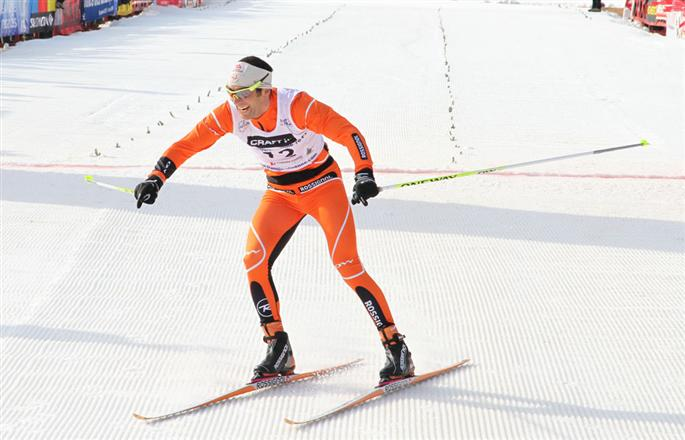
\includegraphics[width=7cm] {fondforme.jpg}
  \end{center}
  \caption{Que préférer?  Le fond, la forme ou les deux ? }
  \label{fig:fondforme}
\end{figure}

\begin{figure}[htpb]
  \begin{center}
    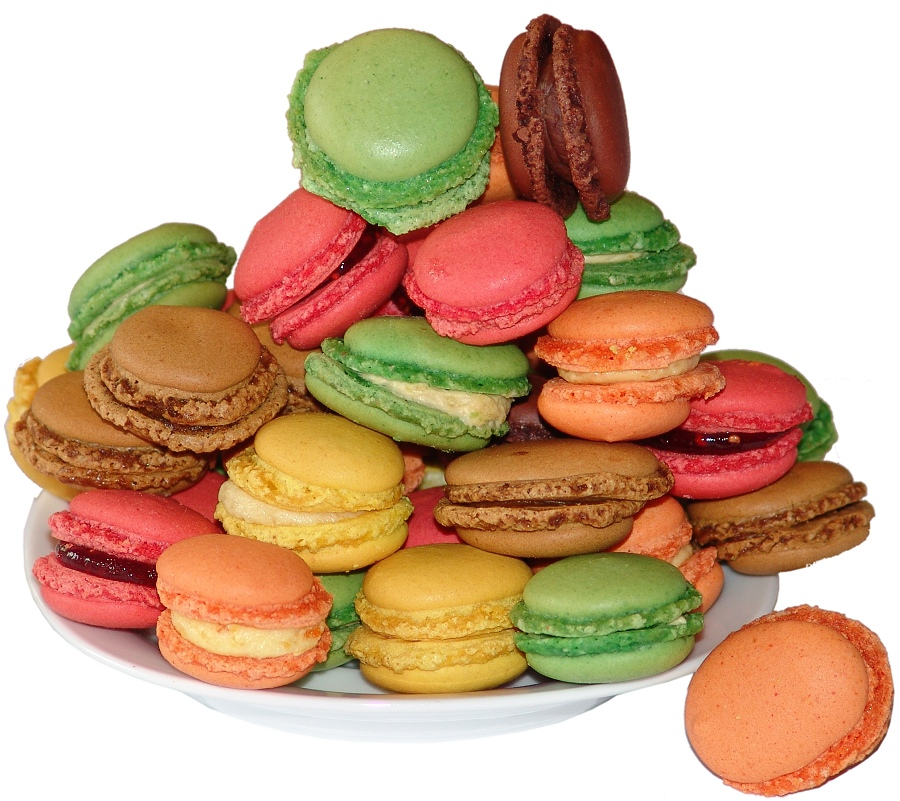
\includegraphics[width=\columnwidth] {gouts.jpg}
  \end{center}
  \caption{Que préférer ? Le goût, la couleur ou les deux ?  }
  \label{fig:gouts}
\end{figure}

Il est possible d'utiliser le mot clé {\texttt cite} pour citer des références
bibliographiques.  

Un premier exemple de \cite{akgu07},\cite{akgu091}\cite{zwic00} \ldots

Il est posssible à l'aide de la commande {\texttt \\url{}} d'insérer un
hyperlien, par exemple : \url{http://en.wikibooks.org/wiki/LaTeX/Command_Glossary}

\section{État de l'Art} 
{\tiny tiny \small small \Small Small \large large \Large Large \Huge Huge}
{\textit
Depuis longtemps, il fixe son précieux sous une forme écrite.
Naguère, caractères faits de plomb, aujourd'hui de photons. Hermès aux semelles de vent. Du lourd au léger.  
Donald Knuth est fils de Guntenberg !\dots
}
\href{http://micro.lemondeinformatique.fr/nouveaux-produits/lire-datatraveler-hyperx-predator-19600.html}{1To}
\section{Méthode}

Ce document vise à agréger en un minimum d'espace, le maximum de possibilités
d'édition avec Latex.

Le document est disponible sur github,  vous pouvez bein sûr le modifier en y ajoutant
vos trouvailles pour en faire profiter tout le monde.

\begin{lstlisting}
git clone https://github.com/buguen/communication.git
\end{lstlisting}

\begin{algorithm}                      % enter the algorithm environment
\label{alg1}                           % and a label for \ref{} commands later in the document
\caption{Determination of signatures list}
\begin{algorithmic}                    % enter the algorithmic environment
\REQUIRE $\mathbf{t}_x$,$\mathbf{r}_x$
\REQUIRE $\mc{G}_s$,$\mc{G}_v$,$\mc{G}_r$
\STATE $\mathcal{L} = \emptyset $ Initialize a list of signatures
\STATE $\mathcal{V}_t \leftarrow \textrm{get visible nodes(}\mc{G}_r,\mathbf{t}_x\textrm{)}$
\STATE $\mathcal{V}_r \leftarrow \textrm{get visible nodes(}\mc{G}_r,\mathbf{r}_x\textrm{)}$
\FOR {$nt \in \mathcal{V}_t$}
\FOR {$nr \in \mathcal{V}_t$}
\STATE $\mc{S}_{it,ir}  = \textrm{Dijkstra}(\mc{G}_v,n_t,n_r)$
\STATE $\mathcal{L}\leftarrow \mathcal{L}.\textrm{append(}\mc{S}_{it,ir}\textrm{)}$
\ENDFOR
\ENDFOR
\end{algorithmic}
\end{algorithm}
\section{Organisation du répertoire template}

\begin{verbatim}

.
| clean
| esir-template.pdf
| esir-template.tex
| figures
| IEEEbib.bst
| IEEEtranfr.cls
| images
|   Gs2.pdf
| README
| ref.bib

\end{verbatim}

\begin{comment}
Ceci est un commentaire. Tout ce qui est écrit ici 
ne sera pas visible dans le document final 
\end{comment}

\begin{figure}[htbp]
\begin{centering}
%\textsf{Une figure A single column figure goes here}
\par
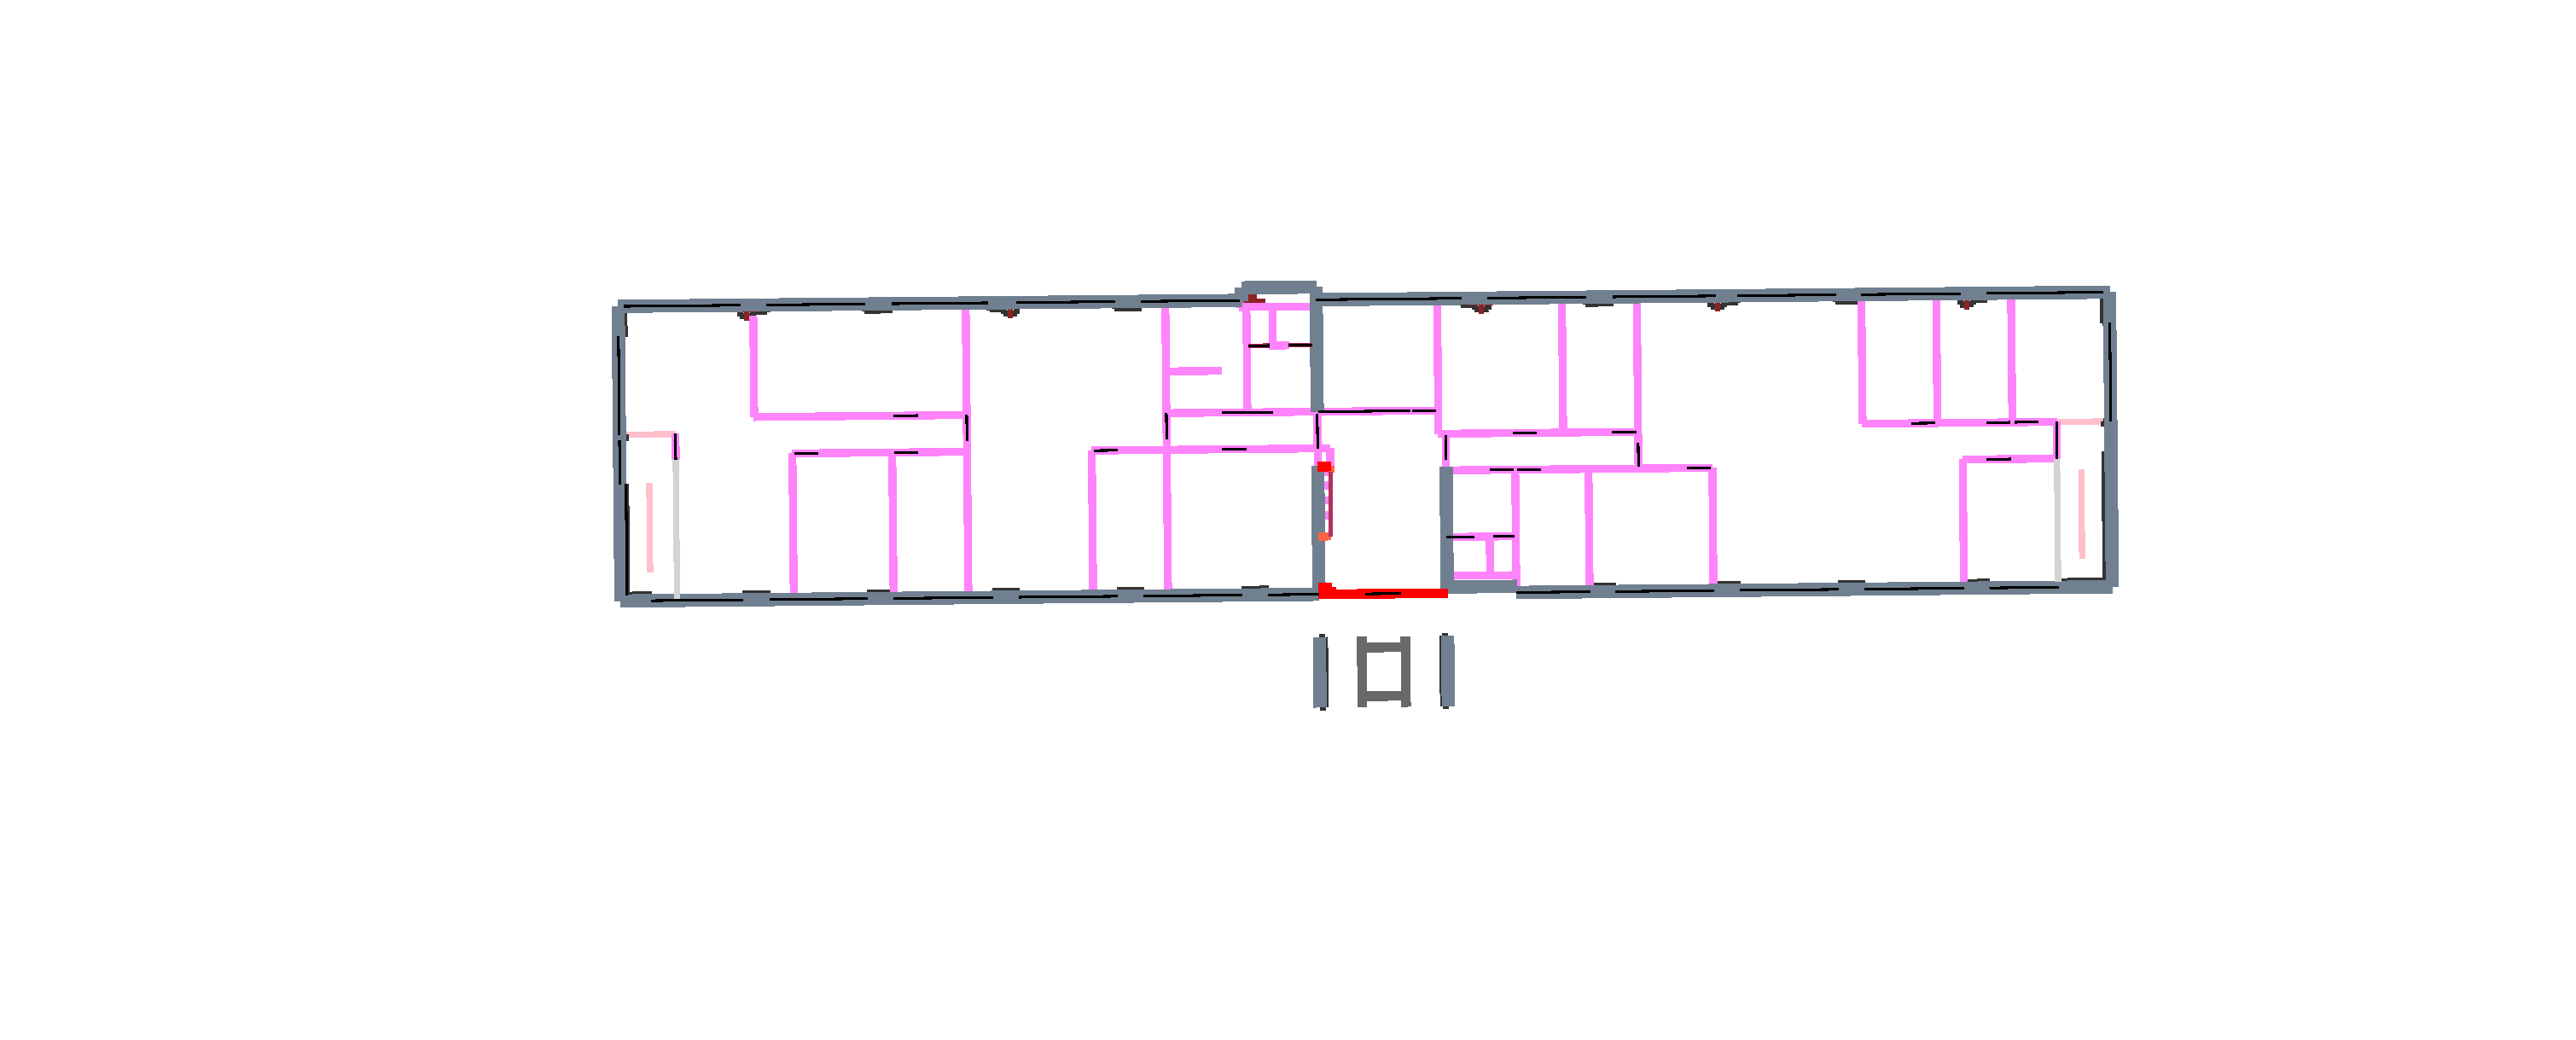
\includegraphics[width=7cm]{Gs2.pdf}
\caption{La légende est \emph{sous} la figure}
\end{centering}
\end{figure}
%



\begin{table}[htbp]
\caption{Cette légende  est \emph{sur} la table}
\centering{}
\begin{tabular}{|c|c|}
\hline 
LAPIN & CHAT \tabularnewline
\hline
\hline 
CHEVAL  & ENCLUME \tabularnewline
\hline
\end{tabular}
\caption{Cette légende  est \emph{sous} la table}
\end{table}
 
\section{Quelques jolies exemples}

\subsection{Poker face}

club, diamond, heart spade
$$\clubsuit, \diamondsuit, \heartsuit ,\spadesuit$$

\subsection{Pile ou Face ? }

La probabilité d'obtenir k fois pile quand on lance $n$ fois la pièce

\begin{equation}
    P(k pile)   = {n \choose k} p^k (1-p)^{ n-k}
\end{equation}

\subsection{Les pépites du copain d'Hardy}

\begin{equation}
  \frac{1}{\Bigl(\sqrt{\phi \sqrt{5}}-\phi\Bigr) e^{\frac25 \pi}} =
    1 + \frac{e^{-2\pi}} 
             {1+\frac{e^{-4\pi}} 
             {1+\frac{e^{-6\pi}}
             {1+\frac{e^{-8\pi}} 
             {1+\ldots} } } }
\end{equation}

\subsection{What else ? }

Les équations de qui déjà ? En tout cas c'est beau et ça sert ?

\begin{equation}
\begin{aligned}
    \nabla \times \vec{\mathbf{B}} -\, \frac1c\,
    \frac{\partial\vec{\mathbf{E}}}{\partial t} & = \frac{4\pi}{c}\vec{\mathbf{j}} \\  
    \nabla \cdot \vec{\mathbf{E}} & = 4 \pi \rho \\
    \nabla \times \vec{\mathbf{E}}\, +\, \frac1c\,
    \frac{\partial\vec{\mathbf{B}}}{\partial t} & = \vec{\mathbf{0}} \\
    \nabla \cdot \vec{\mathbf{B}} & = 0
\end{aligned}
\end{equation}

\section{Conclusion}
\begin{itemize}
  \item {\textbf GERONTE} - Latex c'est frais
  \item {\textbf ALCESTE} - Trop pas  ! Je fais la même chose avec BureauOuvert.org
  \item {\textbf GERONTE} - Mouais \dots
\end{itemize}
%
%\begin{comment}
%\bibliographystyle{IEEEbib}
\bibliographystyle{utphys}
%\bibliographystyle{alpha}
\bibliography{ref}

%\end{comment}
{}
\begin{IEEEbiography}
[{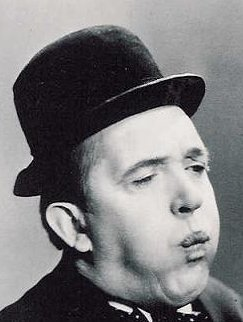
\includegraphics[width=2cm]{SLaurel.jpg}}]
{Stan Laurel } era un actor cómico, escritor y director británico,
famoso por ser miembro del famoso dúo cómico junto a Oliver Hardy 

\end{IEEEbiography}

\begin{IEEEbiography}
[{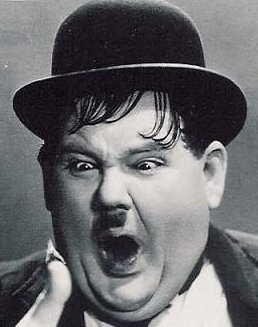
\includegraphics[width=2cm]{OHardy.jpg}}]
{Oliver Hardy} Homonyme du mentor de Srinivasa Ramanujan
\end{IEEEbiography}

\end{document}
